\documentclass{article}
\usepackage[utf8]{inputenc}
\usepackage{tikz}
\usetikzlibrary{positioning}
\usetikzlibrary{shapes}

\begin{document}

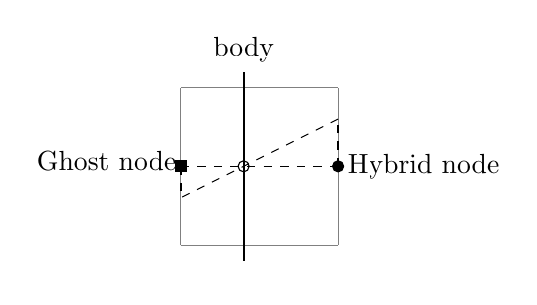
\begin{tikzpicture}
%grid
%horizontal
\draw[gray, thin] (0,0) -- (2,0);
\draw[gray, thin] (0,2) -- (2,2);
%vertical
\draw[gray, thin] (0,0) -- (0,2);
\draw[gray, thin] (2,0) -- (2,2);
%body
\draw[black, thick] (.8,-.2) -- (.8,2.2) node[anchor=south] {body}; 
%extrap lines
\draw[black, thick, dashed] (2,1) -- (2,1.6); %vert right
\draw[black, thick, dashed] (0,1) -- (0,.6);%ver left
\draw[black, dashed] (2,1.6) -- (0,.6);%diag
\draw[black, dashed] (0,1) -- (2,1);%horizontal
%nodes
\draw [black] (.8,1) circle (2pt); %fluid
\filldraw [black] (2,1) circle (2pt) node[anchor=west]{Hybrid node};%hybrid
\filldraw [black] ([xshift=-2pt,yshift=-2pt]0,1) rectangle ++(4pt,4pt) node[anchor=east]{Ghost node}; %ghost

%anchors used to make the pictures align with each other
\draw[white] (-.4,-.4) -- (2.40,-.4) -- (2.4,2.4) -- (-.4,2.4) -- cycle;

\end{tikzpicture}
\end{document}